%Umfang ca. 1-2 Seite
%Was waren die 6 wichtigsten Erfahrungen des Projekt-Teams (3 positive, 3 negative)?
%Nennen Sie stichwortartig die positiven bzw. negativen Erfahrungen und dessen Ursachen (Einflussfaktoren)
%in einem Ishikawa (fishbone) Diagramm

\begin{center}
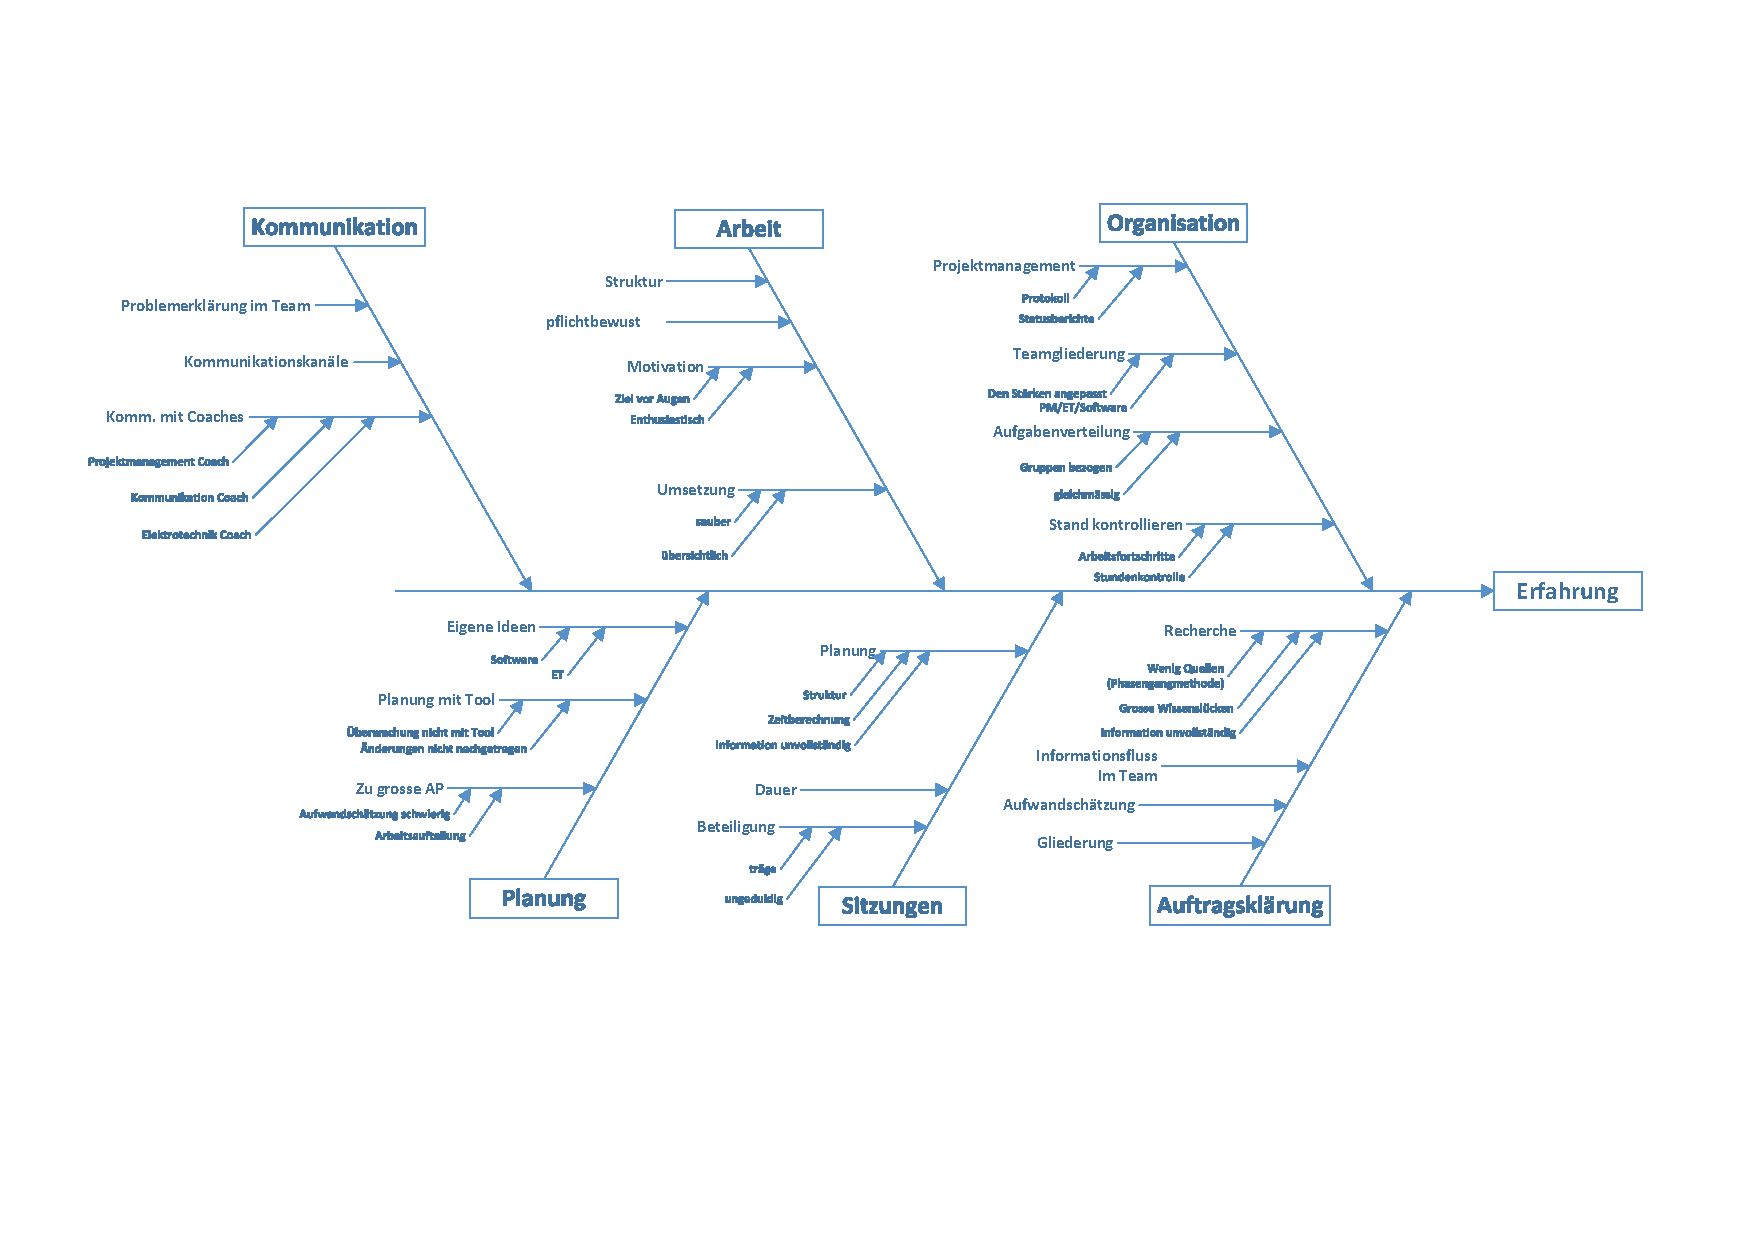
\includegraphics[scale=0.75]{Visio-pmaFishbone}
\newline
Diagramm 1: Ursache-Wirkungs-Diagramm von Projektteam 1.
\end{center}

Das Ursache-Wirkungs-Diagramm [Diagramm 1], auch Ishikawa-Diagramm oder Fishbone genannt, vom gesamten Projekt zeigt je drei positive und drei negative Bereiche im Projekt, die analysiert werden. Im oberen Teil stehen die positiv erfahrenen Bereiche: Kommunikation, Arbeit und Organisation. In der unteren Hälfte stehen die für negativ befundenen Bereiche: Planung, Sitzungen und Auftragsklärung.
Im folgenden Kapitel sind die positiven Bereiche Arbeit und Organisation und die negativen Bereiche Sitzung und Auftragsklärung erklärt und erläutert.